%-------------------------------------------------
\begin{frame}
    \frametitle{Context Mapping}
    Una volta individuati i \textbf{Subdomain} sono state analizzate le possibili relazioni che avvengono tra di essi.

    \bigskip

    In particolare, sono state individuate due tipologie di interazione:
    \begin{itemize}
        \item \textbf{Partnership}: dove i componenti si accordano sull'integrazione delle funzionalità
        \item \textbf{Upstream - Downstream (Conformist)}: dove il downstream si adatta alla specifica api definita dall'upstream
    \end{itemize}

\end{frame}
%------------------------------------------------

%-------------------------------------------------
\begin{frame}
    \frametitle{Context Mapping}

    \begin{figure}[H]
        \centering
        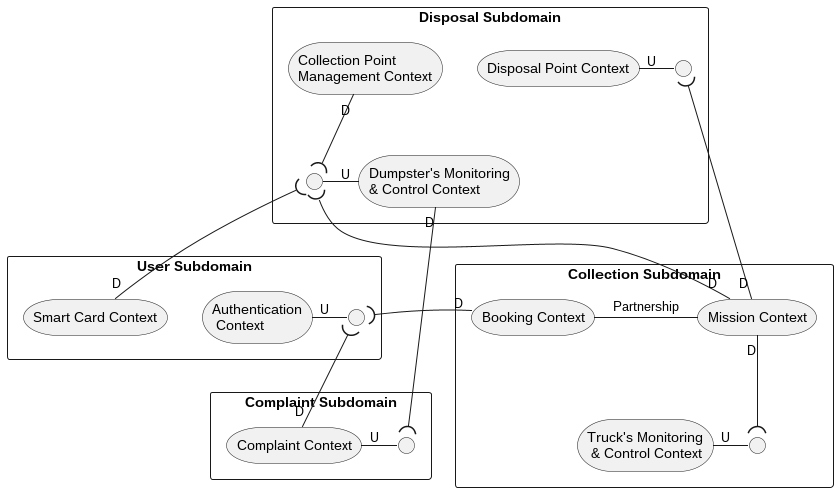
\includegraphics[width=\linewidth]{../img/context-mapping}
    \end{figure}

\end{frame}
%------------------------------------------------